
% ***************************************************
% Example of an internal chapter
% ***************************************************
%This is an internal chapter of the thesis.
%If you have a long title, you can supply an abbreviated version to print in the Table of Contents using the optional argument to the \chapter command.
\chapter[Results]{Results}
\label{Chap:label}	%CREATE YOUR OWN LABEL.
\pagestyle{headings}


To ensure that the firewall was performing properly, a few tests were conducted. In this chapter, the testing results for the performance and the resource utilisation among other features are discussed. 

\section{Modifications}
The design was changed from the 2 ethernet interfaces to a design with just a single ethernet interface. 

\section{Performance}

Talk about wishbone bus speed. 
Initial tests were also conducted at 100MHz, but due to timing issues, it was reverted to 50MHz.


To test the speed of the packet classifier, a Agilent MSO6054A MSO was used (4GSa/s). A pin was set to the output of the crs\_dv of the PHY and the crs\_dv after the packet filter. The time between the rising and falling edge of the output will be the delay added by the packet filter. 


As the shift register in the hardware has a length of 224 bits, at a clock frequency of 50Mhz, the added latency is $224 \times \frac{1}{50\times 10^6} = 4.48 \times 10^{-6} = 4.48uS$. 


\begin{figure}[h!]
    \centering
    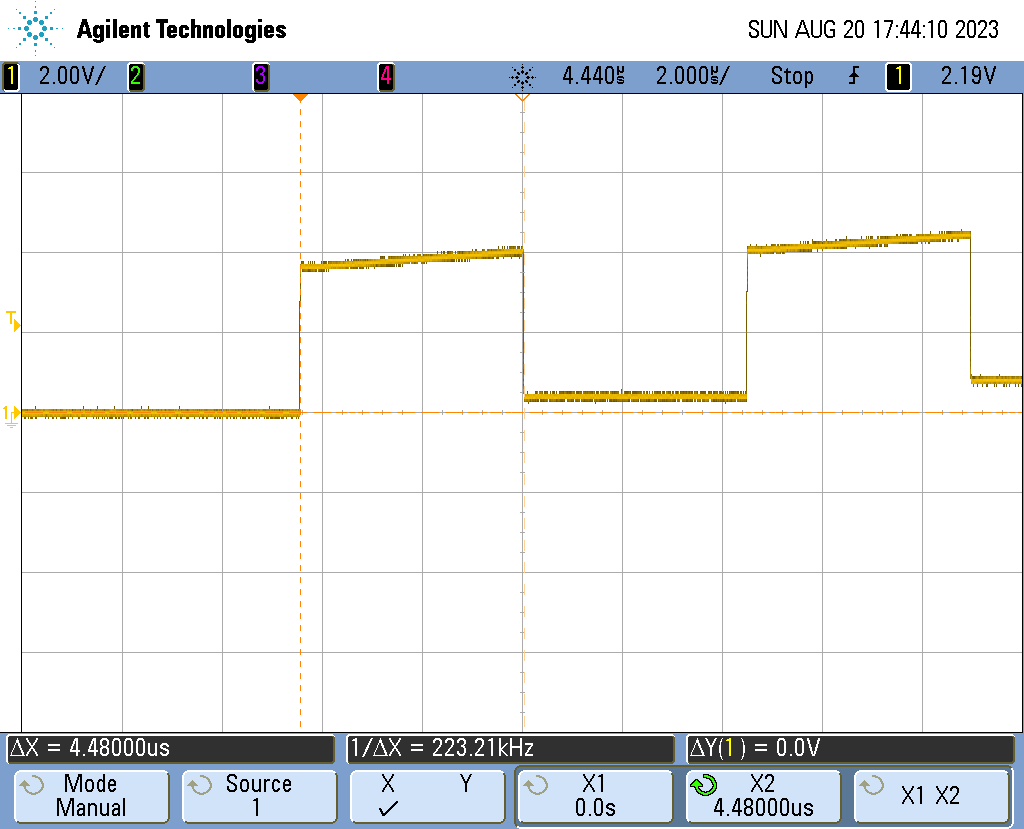
\includegraphics[width=0.75\textwidth]{Images/scope_4.png}
    \caption[Added latency by packet filter waveform]{Added latency by packet filter waveform.}
    \label{fig:packet_classifier_architecture}
\end{figure}

There is two pulses in this graph. This is due to when the crs\_dv line gets disasserted at the end of the packet. From this the time taken to receive the packet can be found to be 8.94uS. This is just an observation and is proportional to the packet size.



The same setup was used to test the preexisting solution, except this time GPIO pins were set high and low. It is assumed that the latency of setting the pin high cancels out with the latency of setting the pin low. 


\subsection{Testing setup}

\subsection{Results}



\section{Ultilisation}

Could be a big section where i take a look at the design against the number of rules - show power usage and gate consumption.


\section{Timing constraints}
\label{sec:timing_constraints}